\section{\large Конструкторская часть}

В  данном  разделе  рассматривается спроектированная база данных, соответствующая выбранной в  аналитической части СУБД, приводится диаграмма базы данных, рассматриваются сценарии создания таблиц БД и основные используемые паттерны проектирования.

Для таблиц необходимо описать информацию о стоблцах (типы данных, ограничения, значения), а также описать связь между описанными таблицами при помощи диаграммы базы данных.

На основе используемых паттернов проектирования и информации о типе базы данных необходимо построить диаграмму классов приложения, на которой будут выделены основные классы и интерфейсы, а также их методы.

\subsection{Диаграмма базы данных}

По полученным выше таблицам, отображающим свойства столбцов таблиц базы данных, построим диаграмму базы данных (\textit{англ. database schema}) при помощи языка разметки баз данных (\textit{англ.} Database Markup Language, DML), предназначенного для представления данных и информации о таблицах, взятых из реляционной базы данных,

Диаграмма базы данных для поставленной задачи отображена на рисунке~\ref{fig:dbdiagram}.

\begin{figure}[h!]
	\centering
	\captionsetup{justification=centering}
	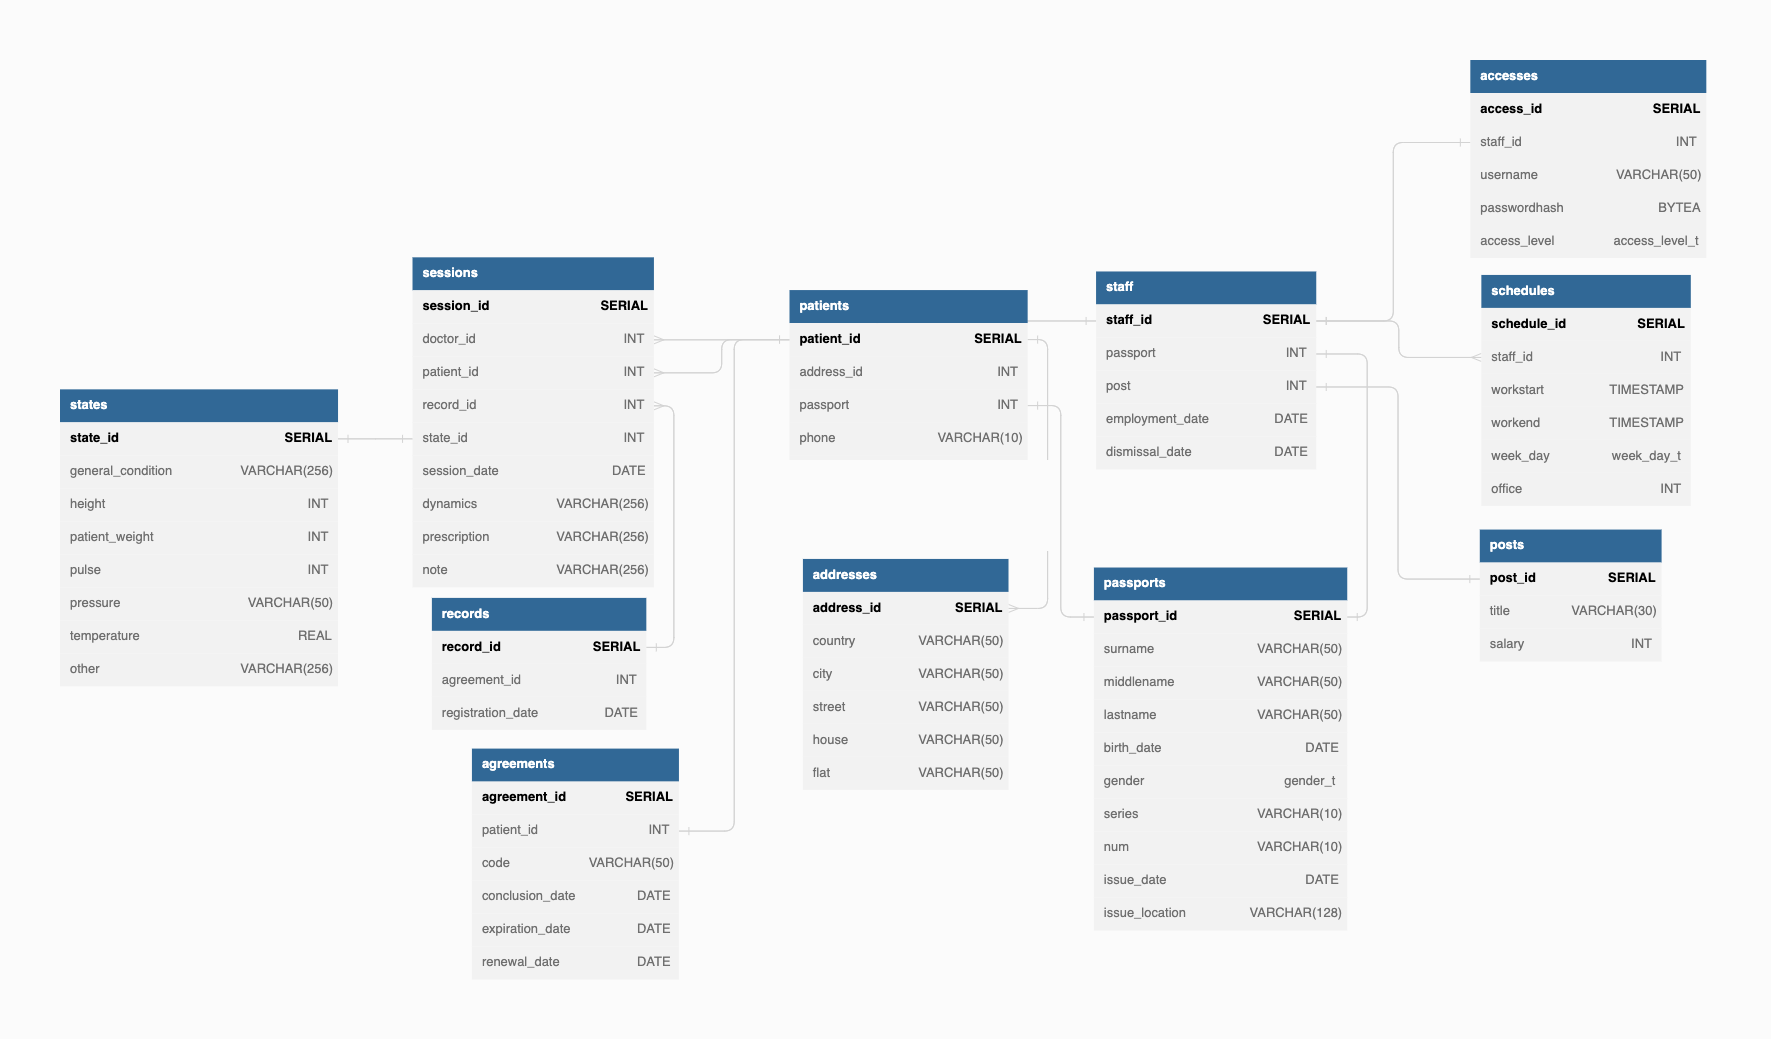
\includegraphics[width=170mm]{dbdiagram.png}
	\caption{Диаграмма базы данных для поставленной задачи}
	\label{fig:dbdiagram}
\end{figure}

\subsection{Таблицы БД}

Для выделенных в аналитической части категорий данных и соответствующей им информации, приведённой в таблице~\ref{table:category-info}, база данных должна содержать следующие таблицы:

\begin{itemize}[leftmargin=1.6\parindent]
	\item[---] пациенты поликлиники --- patients;
	\item[---] сотрудники поликлиники --- staff;
	\item[---] должности в поликлинике --- posts;
	\item[---] приёмы пациентов --- sessions;
	\item[---] расписания --- schedules;
	\item[---] медицинские карты пациентов --- records;
	\item[---] состояния пациентов --- states;
	\item[---] договоры с пациентами --- agreements;
	\item[---] паспорты --- passports;
	\item[---] доступы --- accesses;
	\item[---] адреса --- addresses.
\end{itemize}

Используя знания о выбранной СУБД (PostgreSQL) и приведённую на рисунке~\ref{fig:er} диаграмму сущность-связь, определим для каждой из перечисленных выше таблиц столбцы, их типы и ограничения, в таблицах~\ref{table:patients-columns}~--~\ref{table:addresses-columns}.

\begin{table}[H]
\begin{center}
	\captionsetup{justification=raggedright,singlelinecheck=off,margin=5mm}
	\caption{Информация о столбцах таблицы пациентов поликлиники}
	\begin{tabular}{| c | c | c | c |}
		\hline
		Столбец & Тип данных & Ограничения & Значение \\
		\hline
		patient\_id & SERIAL & \makecell{NOT NULL, \\ PRIMARY KEY} & ID пациента \\
		\hline
		address\_id & INT & \makecell{NOT NULL, \\ FOREIGH KEY} & ID  адреса \\
		\hline
		passport & INT & \makecell{NOT NULL, \\ FOREIGH KEY} & ID паспорта \\
		\hline
		phone & VARCHAR(10) & NOT NULL & Номер телефона \\
		\hline
		home\_phone & VARCHAR(10) & --- & Домаший номер телефона \\
		\hline
		email & VARCHAR(20) & --- & Адрес электронной почты \\
		\hline
	\end{tabular}
	\label{table:patients-columns}
\end{center}
\end{table}

\begin{table}[H]
\begin{center}
	\captionsetup{justification=raggedright,singlelinecheck=off,margin=5mm}
	\caption{Информация о столбцах таблицы сотрудников поликлиники}
	\begin{tabular}{| c | c | c | c |}
		\hline
		Столбец & Тип данных & Ограничения & Значение \\
		\hline
		staff\_id & SERIAL & \makecell{NOT NULL, \\ PRIMARY KEY} & ID сотрудника \\
		\hline
		passport & INT & \makecell{NOT NULL, \\ FOREIGH KEY} & ID паспорта \\
		\hline
		post & INT &  \makecell{NOT NULL, \\ FOREIGH KEY} & ID должности \\
		\hline
		employment\_date & DATE & NOT NULL& Дата наёма \\
		\hline
		dismissal\_date & DATE & --- & Дата увольнения\\
		\hline
	\end{tabular}
	\label{table:staff-columns}
\end{center}
\end{table}

\begin{table}[H]
\begin{center}
	\captionsetup{justification=raggedright,singlelinecheck=off,margin=5mm}
	\caption{Информация о столбцах таблицы должностей в поликлинике}
	\begin{tabular}{| c | c | c | c |}
		\hline
		Столбец & Тип данных & Ограничения & Значение \\
		\hline
		post\_id & SERIAL & \makecell{NOT NULL, \\ PRIMARY KEY} & ID должности \\
		\hline
		title & VARCHAR(30) & NOT NULL & Название должности \\
		\hline
		salary & INT & NOT NULL & Зарплата \\
		\hline
	\end{tabular}
	\label{table:posts-columns}
\end{center}
\end{table}

\begin{table}[H]
\begin{center}
	\captionsetup{justification=raggedright,singlelinecheck=off,margin=5mm}
	\caption{Информация о столбцах таблицы приёмов пациентов}
	\begin{tabular}{| c | c | c | c |}
		\hline
		Столбец & Тип данных & Ограничения & Значение \\
		\hline
		session\_id & SERIAL & \makecell{NOT NULL, \\ PRIMARY KEY} & ID приёма \\
		\hline
		doctor\_id & INT & \makecell{NOT NULL, \\ FOREIGH KEY} & ID принимающего врача \\
		\hline
		patient\_id & INT &  \makecell{NOT NULL, \\ FOREIGH KEY} & ID пациента \\
		\hline
		record\_id &  INT &  \makecell{NOT NULL, \\ FOREIGH KEY} & ID медицинской карты \\
		\hline
		state\_id &  INT &  \makecell{NOT NULL, \\ FOREIGH KEY} & ID состояния\\
		\hline
		session\_date & DATE & --- & Дата приёма\\
		\hline
		dynamics & VARCHAR(256) & --- & Динамика состояния \\
		\hline
		prescription & VARCHAR(256) & --- & Назначение \\
		\hline
		note & VARCHAR(256) & --- & Примечание \\
		\hline
	\end{tabular}
	\label{table:sessions-columns}
\end{center}
\end{table}

\begin{table}[H]
\begin{center}
	\captionsetup{justification=raggedright,singlelinecheck=off,margin=5mm}
	\caption{Информация о столбцах таблицы расписаний}
	\begin{tabular}{| c | c | c | c |}
		\hline
		Столбец & Тип данных & Ограничения & Значение \\
		\hline
		schedule\_id & SERIAL & \makecell{NOT NULL, \\ PRIMARY KEY} & ID расписания \\
		\hline
		staff\_id & INT & \makecell{NOT NULL, \\ FOREIGH KEY} & ID сотрудника \\
		\hline
		workstart & TIMESTAMP & NOT NULL & Дата начала работы\\
		\hline
		workend & TIMESTAMP & NOT NULL & Дата окончания работы \\
		\hline
		week\_day & week\_day\_t & NOT NULL & День недели \\
		\hline
		office & INT  & --- & Кабинет \\
		\hline
	\end{tabular}
	\label{table:schedules-columns}
\end{center}
\end{table}

\begin{table}[H]
\begin{center}
	\captionsetup{justification=raggedright,singlelinecheck=off,margin=5mm}
	\caption{Информация о столбцах таблицы медицинских карт пациентов}
	\begin{tabular}{| c | c | c | c |}
		\hline
		Столбец & Тип данных & Ограничения & Значение \\
		\hline
		record\_id & SERIAL & \makecell{NOT NULL, \\ PRIMARY KEY} & ID мед. карты \\
		\hline
		agreement\_id & INT & NOT NULL & ID договора \\
		\hline
		registration\_date & DATE & NOT NULL & Дата постановки на учёт\\
		\hline
	\end{tabular}
	\label{table:records-columns}
\end{center}
\end{table}

\begin{table}[H]
\begin{center}
	\captionsetup{justification=raggedright,singlelinecheck=off,margin=5mm}
	\caption{Информация о столбцах таблицы состояний пациентов}
	\begin{tabular}{| c | c | c | c |}
		\hline
		Столбец & Тип данных & Ограничения & Значение \\
		\hline
		state\_id & SERIAL & \makecell{NOT NULL, \\ PRIMARY KEY} & ID состояния \\
		\hline
		general\_condition & VARCHAR(256) & --- & Общее состояние \\
		\hline
		height & INT &  --- & Рост пациента, см\\
		\hline
		patient\_weight &  INT &  --- & Вес пациента, кг\\
		\hline
		pulse & INT & --- & \makecell{Частота пульса \\в минуту}\\
		\hline
		pressure & VARCHAR(50) & --- & \makecell{Артериальное \\давление }\\
		\hline
		temperature & REAL & --- & \makecell{Температура, \\градусы Цельсия} \\
		\hline
		other & VARCHAR(256) & --- & Прочее \\
		\hline
	\end{tabular}
	\label{table:states-columns}
\end{center}
\end{table}

\begin{table}[H]
\begin{center}
	\captionsetup{justification=raggedright,singlelinecheck=off,margin=5mm}
	\caption{Информация о столбцах таблицы договоров}
	\begin{tabular}{| c | c | c | c |}
		\hline
		Столбец & Тип данных & Ограничения & Значение \\
		\hline
		agreement\_id & SERIAL & \makecell{NOT NULL, \\ PRIMARY KEY} & ID договора \\
		\hline
		patient\_id & SERIAL & \makecell{NOT NULL, \\ FOREIGN KEY} & ID пациента \\
		\hline
		code & VARCHAR(50) & NOT NULL & Номер договора \\
		\hline
		conclusion\_date & DATE & NOT NULL & \makecell{Дата заключения \\договора}\\
		\hline
		expiration\_date & DATE & NOT NULL & \makecell{Дата окончания\\договора} \\
		\hline
		renewal\_date & DATE & NOT NULL & \makecell{Дата обновления \\договора} \\
		\hline
	\end{tabular}
	\label{table:argreements-columns}
\end{center}
\end{table}

\begin{table}[H]
\begin{center}
	\captionsetup{justification=raggedright,singlelinecheck=off,margin=5mm}
	\caption{Информация о столбцах таблицы адресов}
	\begin{tabular}{| c | c | c | c |}
		\hline
		Столбец & Тип данных & Ограничения & Значение \\
		\hline
		address\_id & SERIAL & \makecell{NOT NULL, \\ PRIMARY KEY} & ID адреса \\
		\hline
		country & VARCHAR(50) & NOT NULL & Страна \\
		\hline
		city & VARCHAR(50) & NOT NULL & Город \\
		\hline
		street & VARCHAR(50) & NOT NULL & Улица \\
		\hline
		house & VARCHAR(50) & NOT NULL & Дом \\
		\hline
		flat & VARCHAR(50) & --- & Квартира \\
		\hline
	\end{tabular}
	\label{table:addresses-columns}
\end{center}
\end{table}

\begin{table}[H]
\begin{center}
	\captionsetup{justification=raggedright,singlelinecheck=off,margin=5mm}
	\caption{Информация о столбцах таблицы паспортов}
	\begin{tabular}{| c | c | c | c |}
		\hline
		Столбец & Тип данных & Ограничения & Значение \\
		\hline
		passport\_id & SERIAL & \makecell{NOT NULL, \\ PRIMARY KEY} & ID паспорта \\
		\hline
		surname & VARCHAR(50) & NOT NULL & Фамилия \\
		\hline
		middlename & VARCHAR(50) & NOT NULL & Имя \\
		\hline
		lastname & VARCHAR(50) & --- & Отчество \\
		\hline
		birth\_date & DATE & NOT NULL & Дата рождения\\
		\hline
		gender & gender\_t & NOT NULL & Пол \\
		\hline
		series & VARCHAR(10) & NOT NULL & Серия \\
		\hline
		num & VARCHAR(10) & NOT NULL & Номер \\
		\hline
		issue\_date & DATE & NOT NULL & Дата выдачи\\
		\hline
		issue\_location & VARCHAR(128) & NOT NULL & Место выдачи \\
		\hline
	\end{tabular}
	\label{table:passports-columns}
\end{center}
\end{table}

\begin{table}[H]
\begin{center}
	\captionsetup{justification=raggedright,singlelinecheck=off,margin=5mm}
	\caption{Информация о столбцах таблицы доступов}
	\begin{tabular}{| c | c | c | c |}
		\hline
		Столбец & Тип данных & Ограничения & Значение \\
		\hline
		access\_id & SERIAL & \makecell{NOT NULL, \\ PRIMARY KEY} & ID доступов \\
		\hline
		staff\_id & INT &  \makecell{NOT NULL, \\ FOREIGN KEY} & ID сотрудника \\
		\hline
		username & VARCHAR(50) & NOT NULL & Логин \\
		\hline
		passwordhash & BYTEA  & NOT NULL & Хэш пароля \\
		\hline
		access\_level & access\_level\_t & NOT NULL & Уровень доступа \\
		\hline
	\end{tabular}
	\label{table:accesses-columns}
\end{center}
\end{table}

\clearpage

Создание пользовательских типов данных, а также таблиц и ограничений для них будет приведено в технологической части. 

%\subsection{Основные паттерны проектирования}

%В данной работе будут использован паттерн проектирования REST, рассмотренный ниже.

%\subsubsection{МVC}
%
%MVC (\textit{англ.} Model View Controller)~\cite{mvc} --- архитектурный паттерн, в основе которого лежат  три понятия: модель, представление и контроллер.
%
%Модель содержит всё информацию состояния, данные и логику приложения, необходимую для ведения базы данных.
%Она представляет собой интерфейс для получения и изменения состояния, а также может отправлять оповещения об изменениях состояния наблюдателем, 
%
%Представление определяет собой отображение модели, и, как правило, получает состояние и данные для отображения непосредственно от модели. 
%
%Контроллер получает данные, вводимые пользователем, определяет их смысл для модели, выполняет операции с моделью и управляет её бизнес-логикой, связывая с представлением.
%\clearpage
%
%Упрощённо можно привести следующие этапы работы приложения, к которым может привести взаимодействие с пользователем:
%\begin{enumerate}[label=\arabic*)]
%	\item пользователь взаимодействует с моделью: представление сообщает контроллеру о том, какая была выполнена операция, контроллер должен обработать это действие;
%	\item контроллер обращается к модели с запросами об изменении состояния: контроллер должен интерпретировать действия пользователя и выполнить необходимые операции с моделью;
%	\item котроллер обращается к представлению с запросом об изменении: когда контроллер получает действие от представления, он может в результате его обработки обратиться к представлению с некоторым запросом на изменение (например, заблокировать некоторые кнопки в интерфейсе);
%	\item модель оповещает представление об изменении состояния (вследствие действий пользователя состояние модели может измениться, о чём модель может уведомить представление);
%	\item представление заправшивает у модели информацию состояния: для корректного отображения данных представление может заправшивать текущее состояние (за которое отвечает модель).
%\end{enumerate}

%\subsection{REST}
%
%REST (\textit{англ.} Representational State Transfer, передача репрезентативного состояния) \cite{rest} --- паттерн проектирования, в основе которого лежит понятие ресурса и его состояния. 
%Каждый ресурс имеет URI (unified resourse identifier), универсальный идентификатор, который позволяет совершать различные действия над данным ресурсом, например, операции создания, чтения, обновления и удаления (CRUD --- create, read, update, delete).
%
%Архитектура REST поддерживает выбранную модель клиент-сервер, причём не требует от сервера хранения какой-либо информации о состоянии клиента в периодах между запросами (всю необходимую для выполения операции информацию клиент передаёт во время запроса).
%Поддерживается возможность кэширования ответов сервера на клиенте с целью ускорения быстродействия программы клиента, что помогает уменьшить нагрузку на клиентских машинах.
%
%При этом программный интерфейс приложения (\textit{англ.} API, application \linebreak programming interface), которым пользуется клиент для осуществления запросов на сервер, может быть унифицирован.
%В этом случае стараются придерживаться трёх основных принципов:
%\begin{enumerate}[label=\arabic*)]
%	\item однозначное идентифицирование ресурсов в запросе;
%	\item использование представления для взаимодействия с ресурсами (представление определяет текущее или желаемое состояние ресурса);
%	\item достаточное количество информации в каждом запросе: каждый отдельно взятый запрос содержит информацию, однозрачно определяющее то, как необходимо обрабатывать и идентифицировать данный запрос.
%\end{enumerate}

%\subsection{Диаграмма классов приложения}
%
%Приложение строится согласно диаграмме классов, приведённой на рисунке \ref{fig:uml}.
%
%\clearpage
%
%\begin{figure}[h!]
%	\centering
%	\captionsetup{justification=centering}
%	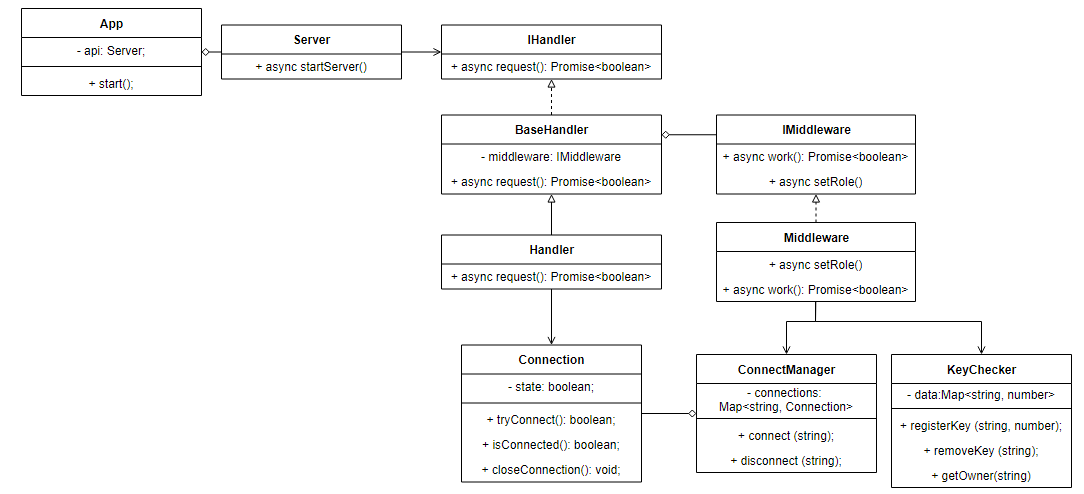
\includegraphics[width=170mm]{uml.png}
%	\caption{Диаграмма классов}
%	\label{fig:uml}
%\end{figure}

\subsection{Описание ролей и доступов}

В соответствии с диаграммой вариантов использования, для использования базы предлагается создать 4 роли: администратор, врач, главный врач и сотрудник регистратуры. 
Администратор будет иметь доступы ко всем таблицам и действиям с ним. 
Главный врач будет иметь доступы ко всем таблицам, кроме таблицы доступов.
Врач будет иметь доступ на все действия для таблиц записей, состояний и приёмов, доступы на чтение для таблиц пациентов и других врачей, а также доступ на чтение и обновление для таблицы расписаний.
Сотрудник регистратуры будет иметь доступы на все действия для таблиц приёмов, расписаний, пациентов и паспортов, а также доступы на чтение в таблицы сотрудников и медицинских карт.

\subsection{Описание организации целостности}

\begin{table}[H]
\begin{center}
	\captionsetup{justification=raggedright,singlelinecheck=off,margin=5mm}
	\caption{Информация об организации целостности таблиц}
	\begin{tabular}{| c | c | c | c | c |}
		\hline
		Таблица & Столбец & Таблица & Столбец & Тип связи \\
		\hline
		states & state\_id & sessions & state\_id & 1 --- 1\\
		\hline
		records & record\_id & sessions & record\_id & 1 --- N \\
		\hline
		records &  agreement\_id & agreements & agreemet\_id & 1 --- 1 \\
		\hline
		patients & patient\_id & sessions & patient\_id & 1 --- N \\
		\hline
		patients & patient\_id & agreements & patient\_id & 1 --- 1\\
		\hline
		patients & patient\_id & addresses & address\_id & 1 --- 1 \\
		\hline
		patients & passport & passports & passport\_id & 1 ---1 \\ \hline
		staff & staff\_id & sessions & session\_id & 1 --- N \\
		\hline
		staff  & staff\_id & accesses & access\_id & 1 --- 1\\
		\hline
		staff  & staff\_id & schedules & staff\_id & 1 --- N\\
		\hline
		staff & passport & passports & passport\_id & 1 --- 1 \\
		\hline
		staff & post & posts & post\_id & 1 --- 1 \\ \hline
	\end{tabular}
	\label{table:passports-columns}
\end{center}
\end{table}

\subsection*{Вывод}

В данном разделе  была рассмотрена спроектированная база данных, соответствующая выбранной в  аналитической части СУБД, приведена диаграмма базы данных, а также рассмотрены сценарии создания таблиц БД и ролевой модели для управления доступом к таблицам.

